\documentclass[tikz,border=0pt]{standalone}
% Shared visual language for the QCSD P3 methodology figures.
\usepackage{tikz}
\usepackage{lmodern}
\usetikzlibrary{arrows.meta,calc,decorations.pathreplacing,positioning,shapes.geometric}

\ifdefined\pdfoutput
  \ifnum\pdfoutput>0
    \ifdefined\pdfinfoomitdate
      \pdfinfoomitdate=1
    \fi
    \ifdefined\pdftrailerid
      \pdftrailerid{}
    \fi
    \ifdefined\pdfsuppressptexinfo
      \pdfsuppressptexinfo=15
    \fi
  \fi
\fi

\definecolor{qink}{HTML}{20242A}
\definecolor{qmid}{HTML}{666A70}
\definecolor{qlight}{HTML}{D7D8DA}
\definecolor{qpale}{HTML}{F2F2F1}
\definecolor{qamber}{HTML}{B8741A}
\definecolor{qamberpale}{HTML}{FFF1D7}
\definecolor{qteal}{HTML}{267985}
\definecolor{qtealpale}{HTML}{E5F2F3}
\definecolor{qred}{HTML}{B44A48}
\definecolor{qredpale}{HTML}{F8E7E6}

\tikzset{
  every node/.style={font=\fontsize{8.6}{10.2}\selectfont,text=qink,align=center},
  flow/.style={draw=qink,line width=.7pt,-{Latex[length=1.8mm,width=1.25mm]}},
  plain flow/.style={draw=qink,line width=.7pt},
  diagnostic/.style={draw=qteal,line width=.85pt,dashed,-{Latex[length=1.8mm,width=1.25mm]}},
  authoritative/.style={draw=qamber,line width=1.05pt,-{Latex[length=1.8mm,width=1.25mm]}},
  failure/.style={draw=qred,line width=.85pt,-{Latex[length=1.8mm,width=1.25mm]}},
  quiet outline/.style={draw=qlight,line width=.55pt,rounded corners=4pt},
  milestone/.style={circle,draw=qink,fill=white,line width=.7pt,inner sep=1.6pt},
  caption/.style={font=\fontsize{8.6}{10.2}\selectfont,text=qink},
  small note/.style={font=\fontsize{7.2}{8.5}\selectfont,text=qmid},
  tiny note/.style={font=\fontsize{6.6}{7.8}\selectfont,text=qmid},
}

% dvisvgm preserves these raw specials when the source is compiled to DVI.
% The PDF build intentionally omits them; its caption supplies the description.
\newcommand{\QCSDSvgMetadata}[2]{%
  \ifdefined\pdfoutput
    \ifnum\pdfoutput=0
      \special{dvisvgm:raw <title>#1</title>}%
      \special{dvisvgm:raw <desc>#2</desc>}%
    \fi
  \else
    \special{dvisvgm:raw <title>#1</title>}%
    \special{dvisvgm:raw <desc>#2</desc>}%
  \fi
}

% Neutral, project-owned pictograms.  They deliberately avoid product marks.
\tikzset{
  pics/client/.style={code={
    \fill[qink] (0,.25) circle (.16);
    \path[fill=qink,rounded corners=2.2pt]
      (-.30,-.30) -- (-.26,.00) arc[start angle=180,end angle=0,radius=.26]
      -- (.30,-.30) -- cycle;
  }},
  pics/tunnel/.style={code={
    \draw[qink,line width=1.1pt,rounded corners=2pt]
      (-.32,-.28) -- (-.32,.04) arc[start angle=180,end angle=0,radius=.32] -- (.32,-.28);
    \draw[qmid,line width=.6pt] (-.20,-.28) -- (-.20,.02)
      arc[start angle=180,end angle=0,radius=.20] -- (.20,-.28);
    \draw[qink,line width=.7pt] (-.36,-.28) -- (.36,-.28);
  }},
  pics/observer/.style={code={
    \draw[qink,line width=.85pt]
      (-.38,0) .. controls (-.17,.25) and (.17,.25) .. (.38,0)
      .. controls (.17,-.25) and (-.17,-.25) .. cycle;
    \fill[qink] (0,0) circle (.09);
  }},
  pics/gateway/.style={code={
    \path[draw=qink,fill=qpale,line width=.75pt,rounded corners=1.5pt]
      (-.34,-.25) rectangle (.34,.25);
    \draw[qink,line width=.65pt] (-.20,.03) -- (.20,.03);
    \fill[qink] (-.20,-.12) circle (.025);
    \fill[qink] (-.08,-.12) circle (.025);
    \fill[qink] (.04,-.12) circle (.025);
    \draw[qink,line width=.65pt] (.22,.25) -- (.22,.40);
  }},
  pics/server/.style={code={
    \path[draw=qink,fill=qpale,line width=.75pt]
      (-.27,-.36) rectangle (.27,.36);
    \draw[qmid,line width=.5pt] (-.18,.20) -- (.18,.20)
      (-.18,.02) -- (.18,.02) (-.18,-.16) -- (.18,-.16);
    \fill[qink] (.15,.27) circle (.022);
    \fill[qink] (.15,.09) circle (.022);
    \fill[qink] (.15,-.09) circle (.022);
  }},
  pics/globe/.style={code={
    \draw[qink,line width=.7pt] (0,0) circle (.31);
    \draw[qmid,line width=.45pt] (-.31,0) -- (.31,0);
    \draw[qmid,line width=.45pt] (0,-.31) .. controls (-.16,-.14) and (-.16,.14) .. (0,.31);
    \draw[qmid,line width=.45pt] (0,-.31) .. controls (.16,-.14) and (.16,.14) .. (0,.31);
  }},
  pics/capture/.style={code={
    \path[draw=qink,fill=white,line width=.65pt]
      (-.27,-.34) -- (-.27,.34) -- (.10,.34) -- (.27,.17) -- (.27,-.34) -- cycle;
    \draw[qmid,line width=.5pt] (.10,.34) -- (.10,.17) -- (.27,.17);
    \draw[qmid,line width=.55pt] (-.16,.08) -- (.15,.08)
      (-.16,-.04) -- (.08,-.04) (-.16,-.16) -- (.15,-.16);
  }},
  pics/dataset/.style={code={
    \path[draw=qink,fill=white,line width=.65pt] (-.31,-.25) rectangle (.25,.28);
    \path[draw=qmid,fill=white,line width=.5pt] (-.22,-.34) rectangle (.34,.19);
    \draw[qmid,line width=.5pt] (-.13,.10) -- (.13,.10)
      (-.13,-.02) -- (.20,-.02) (-.13,-.14) -- (.12,-.14);
  }},
  pics/classifier/.style={code={
    \foreach \y in {-.23,0,.23} { \fill[qink] (-.28,\y) circle (.045); }
    \foreach \y in {-.14,.14} { \fill[qink] (0,\y) circle (.045); }
    \foreach \y in {-.23,0,.23} { \fill[qink] (.28,\y) circle (.045); }
    \foreach \a in {-.23,0,.23} { \foreach \b in {-.14,.14}
      { \draw[qmid,line width=.35pt] (-.235,\a) -- (-.045,\b); } }
    \foreach \a in {-.14,.14} { \foreach \b in {-.23,0,.23}
      { \draw[qmid,line width=.35pt] (.045,\a) -- (.235,\b); } }
  }},
}


\begin{document}
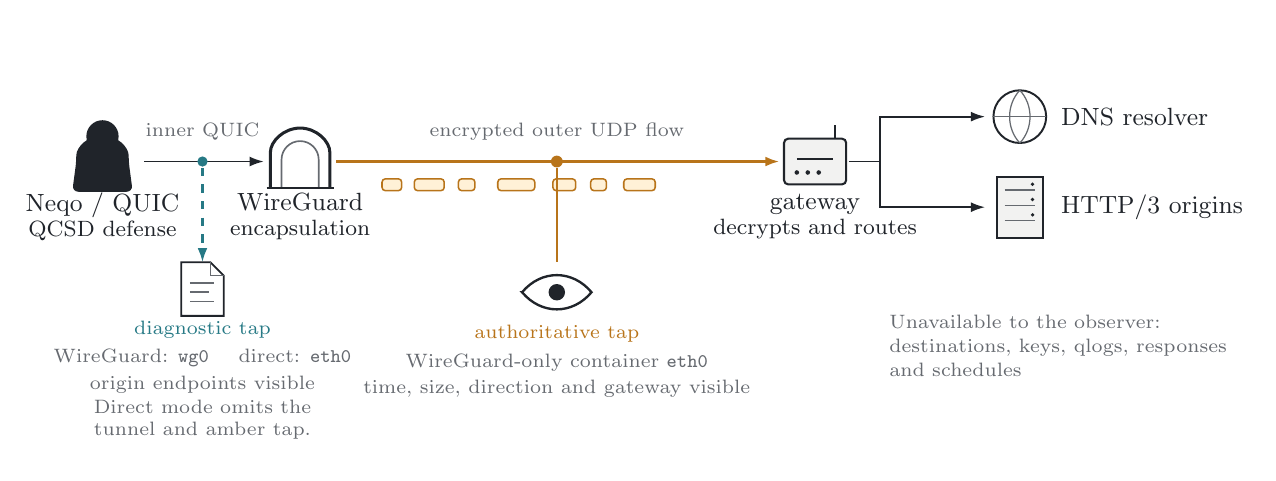
\begin{tikzpicture}[x=1cm,y=1cm]
  \QCSDSvgMetadata
    {QCSD passive observer and capture taps}
    {The WireGuard classification path has a diagnostic tap before encapsulation and an authoritative passive observer on the encrypted outer flow. Direct mode uses container eth0 for the diagnostic tap and omits WireGuard and the outer tap.}
  \path[use as bounding box] (0,0) rectangle (15.5,5.4);

  \pic[scale=1.28] at (.95,3.70) {client};
  \node[caption] at (.95,3.00)
    {Neqo / QUIC\\[-1pt]\footnotesize QCSD defense};

  \draw[flow] (1.48,3.70) -- (3.00,3.70);
  \node[small note,above=4pt] at (2.22,3.70) {inner QUIC};
  \fill[qteal] (2.22,3.70) circle (.065);
  \draw[diagnostic] (2.22,3.62) -- (2.22,2.42);
  \pic[scale=1.00] at (2.22,2.08) {capture};
  \node[small note,text=qteal] at (2.22,1.56) {diagnostic tap};
  \node[tiny note] at (2.22,1.20)
    {WireGuard: \texttt{wg0} \quad direct: \texttt{eth0}};
  \node[tiny note] at (2.22,.86) {origin endpoints visible};
  \node[tiny note,text width=4.3cm] at (2.22,.42)
    {Direct mode omits the tunnel and amber tap.};

  \pic[scale=1.18] at (3.46,3.70) {tunnel};
  \node[caption] at (3.46,3.00)
    {WireGuard\\[-1pt]\footnotesize encapsulation};

  \draw[authoritative] (3.92,3.70) -- (9.55,3.70);
  \node[small note,above=4pt] at (6.72,3.70)
    {encrypted outer UDP flow};
  \foreach \x/\w in {4.50/.25,4.91/.38,5.47/.21,5.97/.47,6.67/.29,7.15/.20,7.57/.40}
    \draw[qamber,fill=qamberpale,line width=.55pt,rounded corners=1.2pt]
      (\x,3.33) rectangle ++(\w,.15);

  \fill[qamber] (6.72,3.70) circle (.075);
  \draw[qamber,line width=.9pt] (6.72,3.62) -- (6.72,2.42);
  \pic[scale=1.16] at (6.72,2.04) {observer};
  \node[small note,text=qamber] at (6.72,1.51)
    {authoritative tap};
  \node[tiny note] at (6.72,1.15)
    {WireGuard-only container \texttt{eth0}};
  \node[tiny note] at (6.72,.81)
    {time, size, direction and gateway visible};

  \pic[scale=1.16] at (10.00,3.70) {gateway};
  \node[caption] at (10.00,3.00)
    {gateway\\[-1pt]\footnotesize decrypts and routes};
  \coordinate (fork) at (10.82,3.70);
  \draw[plain flow] (10.43,3.70) -- (fork);
  \draw[flow] (fork) |- (12.16,4.27);
  \draw[flow] (fork) |- (12.16,3.12);
  \pic[scale=1.08] at (12.60,4.27) {globe};
  \node[caption,anchor=west] at (13.00,4.27) {DNS resolver};
  \pic[scale=1.08] at (12.60,3.12) {server};
  \node[caption,anchor=west] at (13.00,3.12) {HTTP/3 origins};

  \node[small note,anchor=west,align=left,text width=4.6cm] at (10.82,1.36)
    {Unavailable to the observer:\\destinations, keys, qlogs, responses and schedules};
\end{tikzpicture}
\end{document}
